\documentclass{article}
\usepackage[utf8]{inputenc}
\usepackage[T1]{fontenc}
\usepackage{imakeidx}
\usepackage{amsmath}
\usepackage{amssymb}
\usepackage{graphicx}

\graphicspath{ {images/} }

\makeindex
\title{Quantum Computing Explained Solutions}
\author{Ricardo Alcaraz Fraga}
\date{February 2021}

\begin{document}

\begin{titlepage}
\maketitle
\end{titlepage}

\tableofcontents
\clearpage

\section{Introduction}
This document has the intention to show the solutions to the exercises presented in Quantum Computing Explained by David McMahon, the exercies are explained and in some cases R or Python code is presented.

\section{A brief introduction to information theory}
\textbf{1.1} How many bits are necessary to represent the alphabet using a binary code if we only allow uppercase characters? How about if we allow both uppercase and lowercase character?\\ \\
\textbf{Solution}\\
Let's consider that \textit{n} is the number of characters in an alphabet, we would need \textit{x} bits so that \\ 

\begin{center}
$2^x \geq n$\\
$x \geq \log_2 n$\\
\end{center}
The english alphabet has 26 characters, so $n=26$, therefore\\
\begin{center}
$\log_2 26 \approx 4.7$
\end{center}
And since we can't  have 4.7 bits we have to take the next integer, that is 5.\\
\begin{center}
$\therefore{}$ We need 5 bits
\end{center}
How about if we allow both uppercase and lowercase characters? This implies that $n=26 * 2 = 52$ characters. We could solve same equations as above, or we can just remember that\\
\begin{center}
$2^{x + 1} = 2 * 2^x$
\end{center}
Knowing this we can see that\\
\begin{center}
$2^6 \geq 52$\\
$64 \geq 52$\\
$\therefore{}$ We need 6 bits
\end{center}
\textbf{1.2} Describe how you can create an OR gate using NOT gates and AND gates.\\ \\
\textbf{Solution}\\
To create a 1 bit OR gate we need 2 NOT gates and a NAND gate (which is an AND gate followed by a NOT gate), this gates have to be connected as follows (the not gates are going to be created with a NAND gate which receives the signal two times)\\ \\
\begin{center}
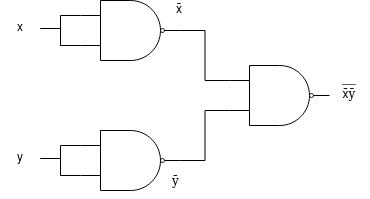
\includegraphics[scale = 0.75]{or using nands.png}
\end{center}
We can see that the result of the circuit is $\overline{\overline{x} \ \overline{y}}$. To develop this we have to remember one Boole's Algebra rule
\begin{center}
$\overline{xy} = \overline{x} + \overline{y}$
\end{center}
Using this rule we can see that \\
\begin{center}
$\overline{\overline{x} \ \overline{y}} = \overline{\overline{x}} + \overline{\overline{y}}$\\
$\overline{\overline{x}} + \overline{\overline{y}} = x + y$
\end{center}
\textbf{1.3} A kilobyte is 1024 bytes. How many messages can it store?\\ \\
\textbf{Solution}\\
This is a very straight forward solution, all that we have to remember is\\
\begin{center}
$1 byte = 8 bits$\\
$1024 bytes= 1024 * 8 = 8192 bits$\\
$\therefore{}$ $1 kilobyte$ can store $2^{8192} messages$
\end{center}
\textbf{1.4} What is the entropy associated with the tossing of a fair coin?\\ \\
\textbf{Solution}\\
Let's remember that a fair coin implies the following\\
\begin{center}
$P(\{heads\}) = P(\{tails\}) = 0.5$
\end{center}
So, being $X$ the event of tossing a fair coin\\
\begin{center}
$H(X) = -\sum p_i \log_2 p_i$\\
$= -(0.5 \log_2 0.5 + 0.5 \log_2 0.5)$\\
$= -(-0.5 - 0.5)$\\
$=1$
\end{center}
\textbf{1.5} Suppose that $X$ consists of the characters A, B, C, D that occur in a signal with respective probabilities 0.1, 0.4, 0.25, 0.25, what is  the Shanon's entropy?\\ \\
\textbf{Solution}\\
Given the probabilities \\
\begin{center}
$P(\{A\}) = 0.1$\\
$P(\{B\}) = 0.4$\\
$P(\{C\}) = 0.25$\\
$P(\{D\}) = 0.25$\\
\end{center}
The Shanon's entropy is the following\\
\begin{center}
$H(X) = - \sum p_i log_2 p_i$\\
$= -(0.1 \log_2 0.1 + 0.4 \log_2 0.4 + 0.25 \log_2 0.25 + 0.25 \log_2 0.25)$
$= -(0.332 - 0.528 - 0.5 - 0.5)$\\
$= 1.86$
\end{center}
\textbf{1.6} A room full of people has incomes distributed in the following way\\ \\
$n(25.5) = 3$\\
$n(30) = 5$\\
$n(42) = 7$\\
$n(50) = 3$\\
$n(63) = 1$\\
$n(75) = 2$\\
$n(90) = 1$\\ \\
What is the most probable income? What is the average income? What is the variance of this distribution?\\ \\
\textbf{Solution}\\
Starting by the most probable income, we can calculate the probability of all incomes, but we don't  have to, knowing that the total people $n = 22$, we can see that the probability of an income is\\
\begin{center}
$\frac{n_j}{n}$
\end{center}
Where $n_j$ is the count of occurences of that income, so the higher the occurences the higher the probability, knowing that the higher occurence is 7, $n(42)$ is the most probable income with a value of $\frac{7}{22}$.\\
The average income is given by the expresion \\
\begin{center}
$\mu = \sum j p_j$\\
$= 25.5(0.13) + 30(0.22) + 42(0.31) + 50(0.13) + 63(0.04) + 75(0.09) + 90(0.04)$\\
$= 44.25$
\end{center}
The variance of the distribution can be calculated in many ways, but I'm going to use the next formula\\
\begin{center}
$\sigma^2 = \frac{\sum X^2}{N} - \mu^2$
\end{center}
Where $X$ is the random variable, N is the number of observations, and $\mu$ is the mean of the distribution. Therefore, the variance  is\\
\begin{center}
$\sigma^2 = \frac{1}{22}(1950.75 + 4500 + 12348 + 7500 + 3969 + 11250 + 8100) - 44.25^2$\\
$= 2255.3522 - 1958.0625 = 297.289$
\end{center}



\printindex
\end{document}
